\chapter{Use Case Definition - Connected Cabin System}
\label{chap:Use Case Definition - Connected Cabin System}
% TODO: (aver) What about moving this to the design and architecture section, instead of having it as a separate
% chapter?

\begin{figure}
	\begin{center}
		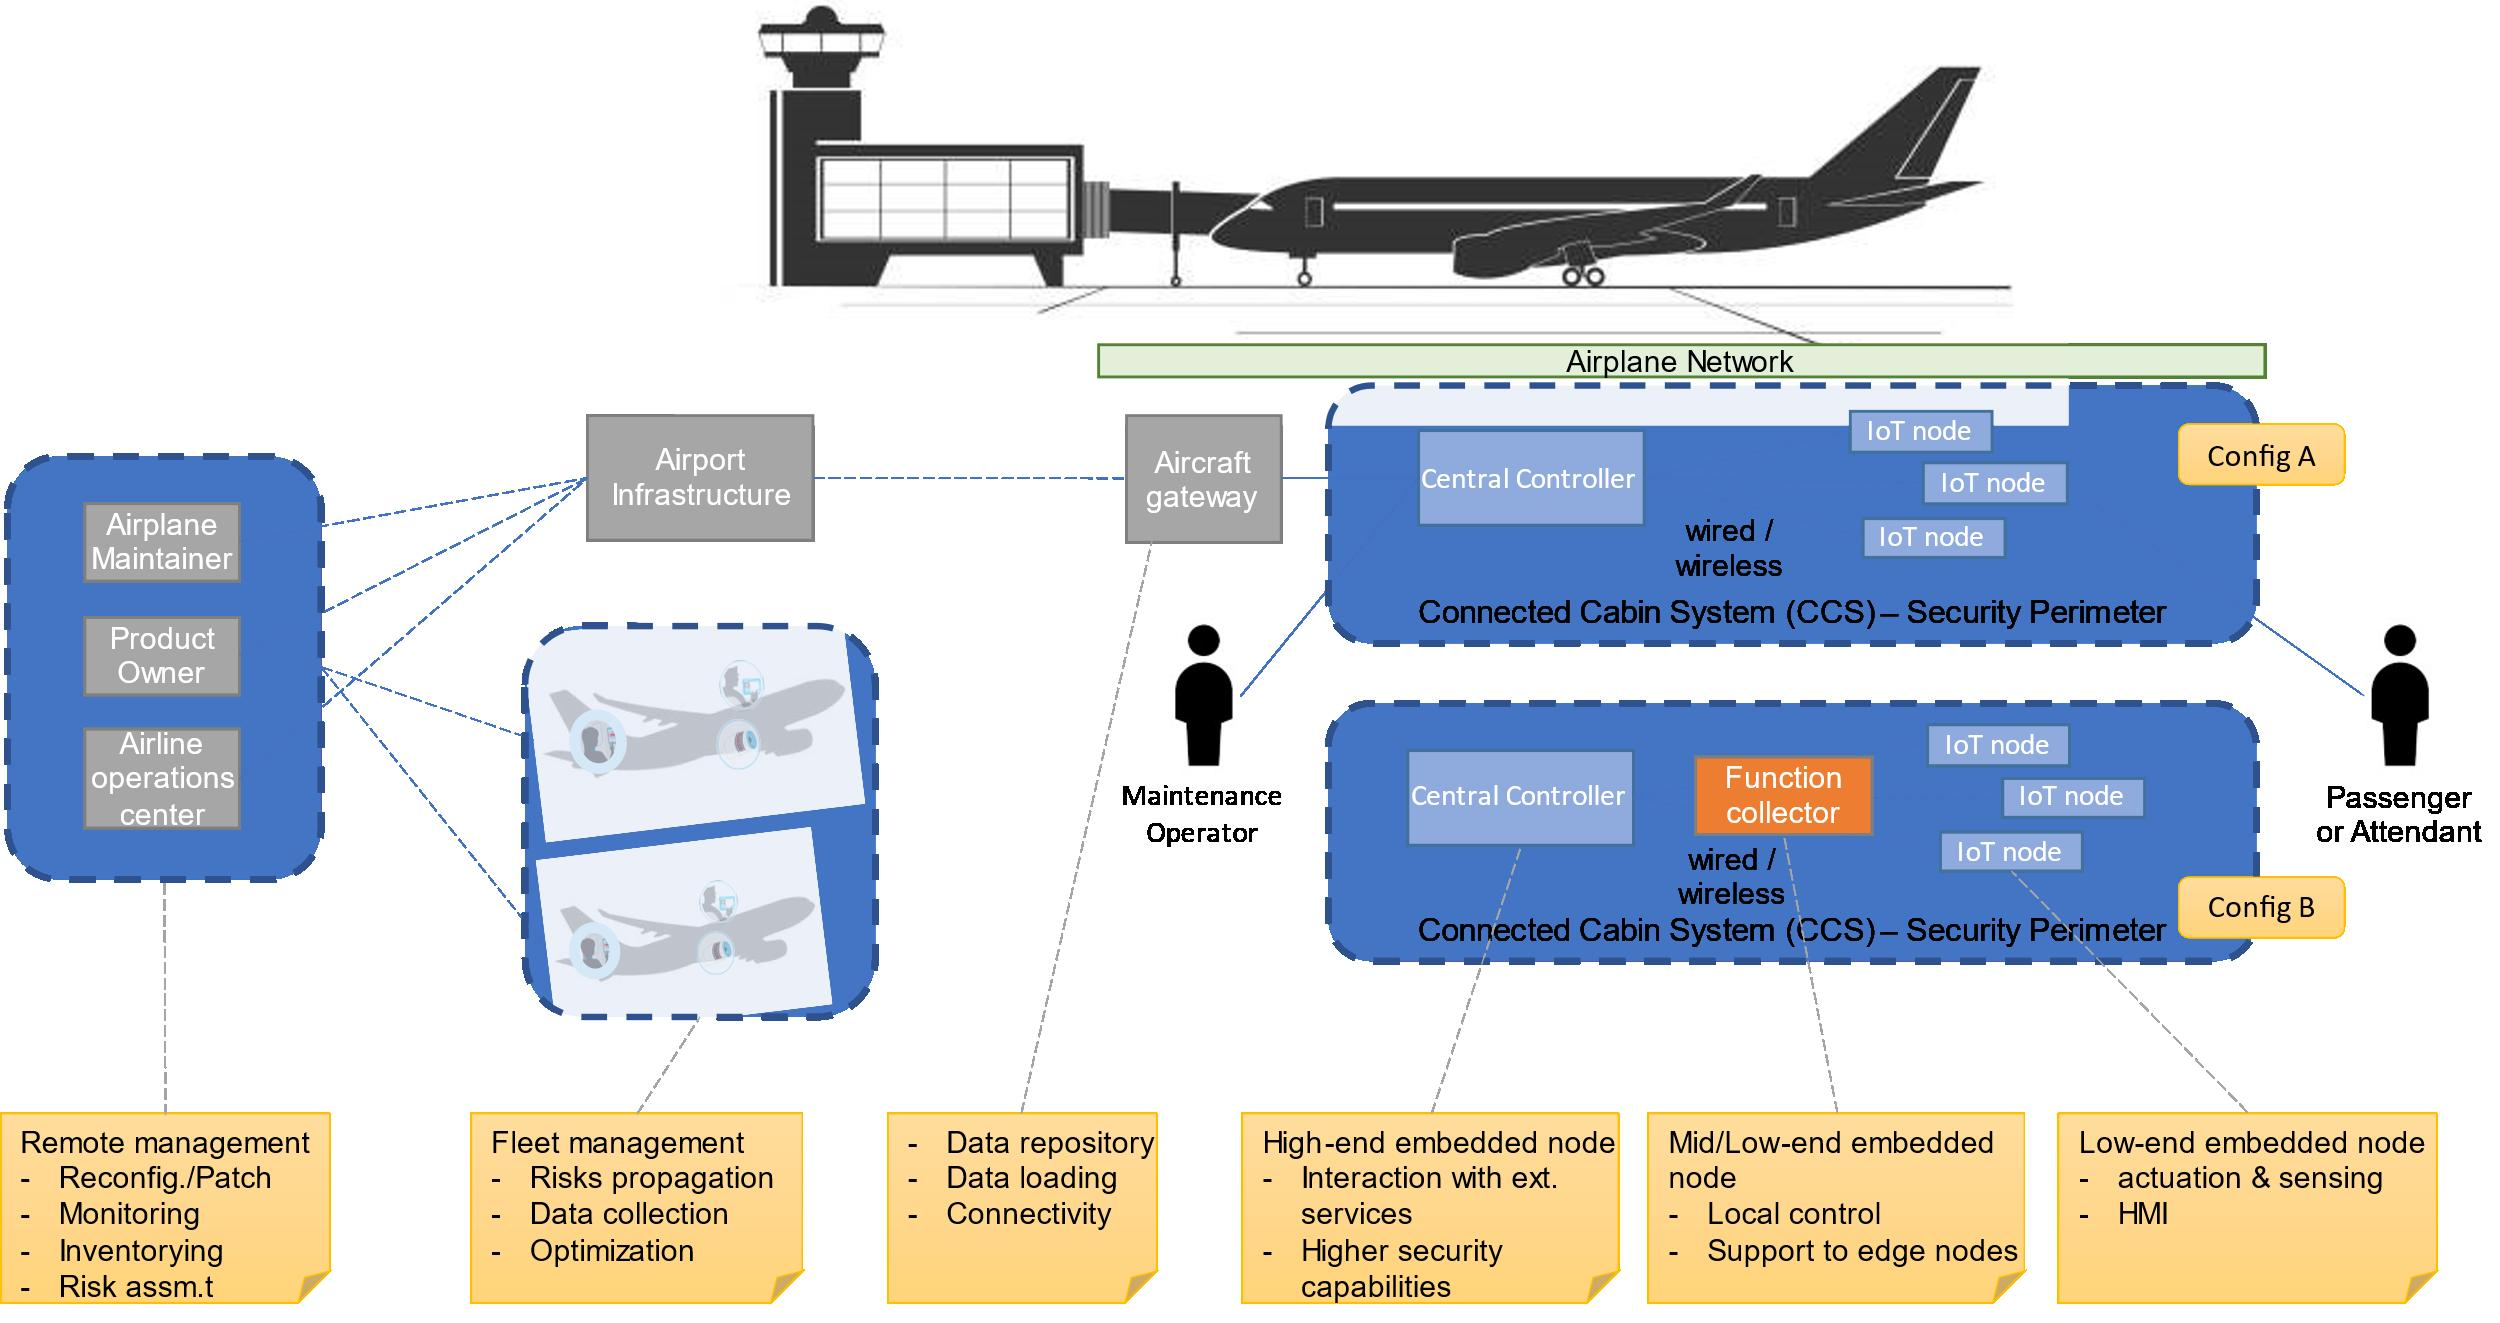
\includegraphics[width=0.95\textwidth]{figures/collins-ccs.jpg}
	\end{center}
	\caption{Collins CCS}
	\label{fig:Collins CCS}
\end{figure}

\section{Background} % (fold)
\label{sec:Background}

Our use case will take the CCS scenario from Figure~\ref{fig:Collins CCS} into consideration and build up on their use
cases, which were borrowed from the CERTIFY project \cite{certifyproject2023}.

Nowadays more and more IoT devices are being deployed to aircraft cabins to improve passenger experience and airline
operations. Benefits span from remote PHM to reduced maintenance time, while also supporting a
continuous (re)certification process. % TODO: (aver) add source, maybe from certify

% section Background (end)

\section{Actors} % (fold)
\label{sec:Actors}

We will consider following actors for our use case.

\begin{itemize}
	\item Airline:
	      Owns the aircraft and oversees daily interactions and systems operations.
	\item Airplane maintainer: They could be e.g., the airplane manufacturer. Oversees maintenance of the aircraft,
	      including the integration of systems designed by different manufacturers and their configuration.
	\item Product Owner: Oversees design and maintenance of systems deployed in the aircraft on assignment of the
	      airplane maintainer.
	\item Maintenance operator: They work for the airplane maintainer. Their responsibilities include e.g.,
	      the replacement of devices or on-site software upgrades of e.g., portable data loaders.
	\item Passenger, Attendant, Pilot: They interact with the aircraft through sensors, actuators or HMI.
\end{itemize}

% section Actors (end)

\section{System Components} % (fold)
\label{sec:System Components}

We will consider an aircraft to have multiple networks, covering various aspects.
\begin{itemize}
	\item In-flight entertainment system
	\item Aircraft System
	\item Flight Maintenance
\end{itemize}

For our use case we will assume config 'A' as the main configuration of the networks, where edge nodes are connected to
a central controller that manages the edge nodes as a subnet.
\begin{itemize}
	\item IoT / Edge Nodes: low-end devices, including actuation, sensing or HMI capabilities, with limited
	      room for hardware and software based cybersecurity, that requires offloading to a more capable
	      instance.
	\item Central Controller: High-end devices with ability to host full-fledged security functionalities.
\end{itemize}

External communication will take place through aircraft gateway offering services for data repository, data loading and
connectivity with external environment. The airline operations center, product owner and airplane maintainer can interact
through the airport infrastructure. A technician may directly access the aircraft if necessary.

% section System Components (end)


\section{Scenarios} % (fold)
\label{sec:Scenarios}

\subsection{Installation of Connected Cabin Systems} % (fold)
\label{sub:Installation of Connected Cabin Systems}

\begin{table}
	\caption{Actors involved}
	\label{tab:Actors involved installation}
	\begin{center}
		\begin{tabular}{ |p{2.5cm}|p{2.5cm}|p{2.5cm}|p{2.5cm}|p{2.5cm}| }
			\hline
			Airline & Airplane Maintainer & Product Owner & Maintenance Operator & Passenger, Attendant, Pilot \\
			\hline
			X       & X                   & X             & X                    & X                           \\
			\hline
		\end{tabular}
	\end{center}
\end{table}

\begin{table}
	\caption{Lifecycle stages involved}
	\label{tab:Lifecycle stages involved installation}
	\begin{center}
		\begin{tabular}{ |c|c|c|c|c| }
			\hline
			Bootstrapping & Operation & Update & Repurposing & Decommissioning \\
			\hline
			X             & -         & X      & -           & X               \\
			\hline
		\end{tabular}
	\end{center}
\end{table}


\subsubsection{Goals}

The goals of this scenario include bootstrapping and customization of devices for specific deployment, updating and
decommissioning of previous systems, guaranteeing a reset to a known and fresh, wiped data, state.
Table~\ref{tab:Actors involved installation} highlights the involved actors and
Table~\ref{tab:Lifecycle stages involved installation} shows the stages involved in this scenario.

\subsubsection{Pre-condition}

In order for this scenario to be valid, following pre-conditions need to be met:
\begin{itemize}
	\item Actors involved can establish a secure connection with the aircraft, wireless or wired, through airport
	      infrastructure
	\item Airport and Aircraft network infrastructure can receive authorization requests for needed connections from
	      the external environment.
	\item The Maintenance Operator is provided access to the airplane and to maintenance ports of the target CCS.

\end{itemize}

\subsubsection{Sub-Scenario 1: Component Installation}

\begin{figure}
	\begin{center}
		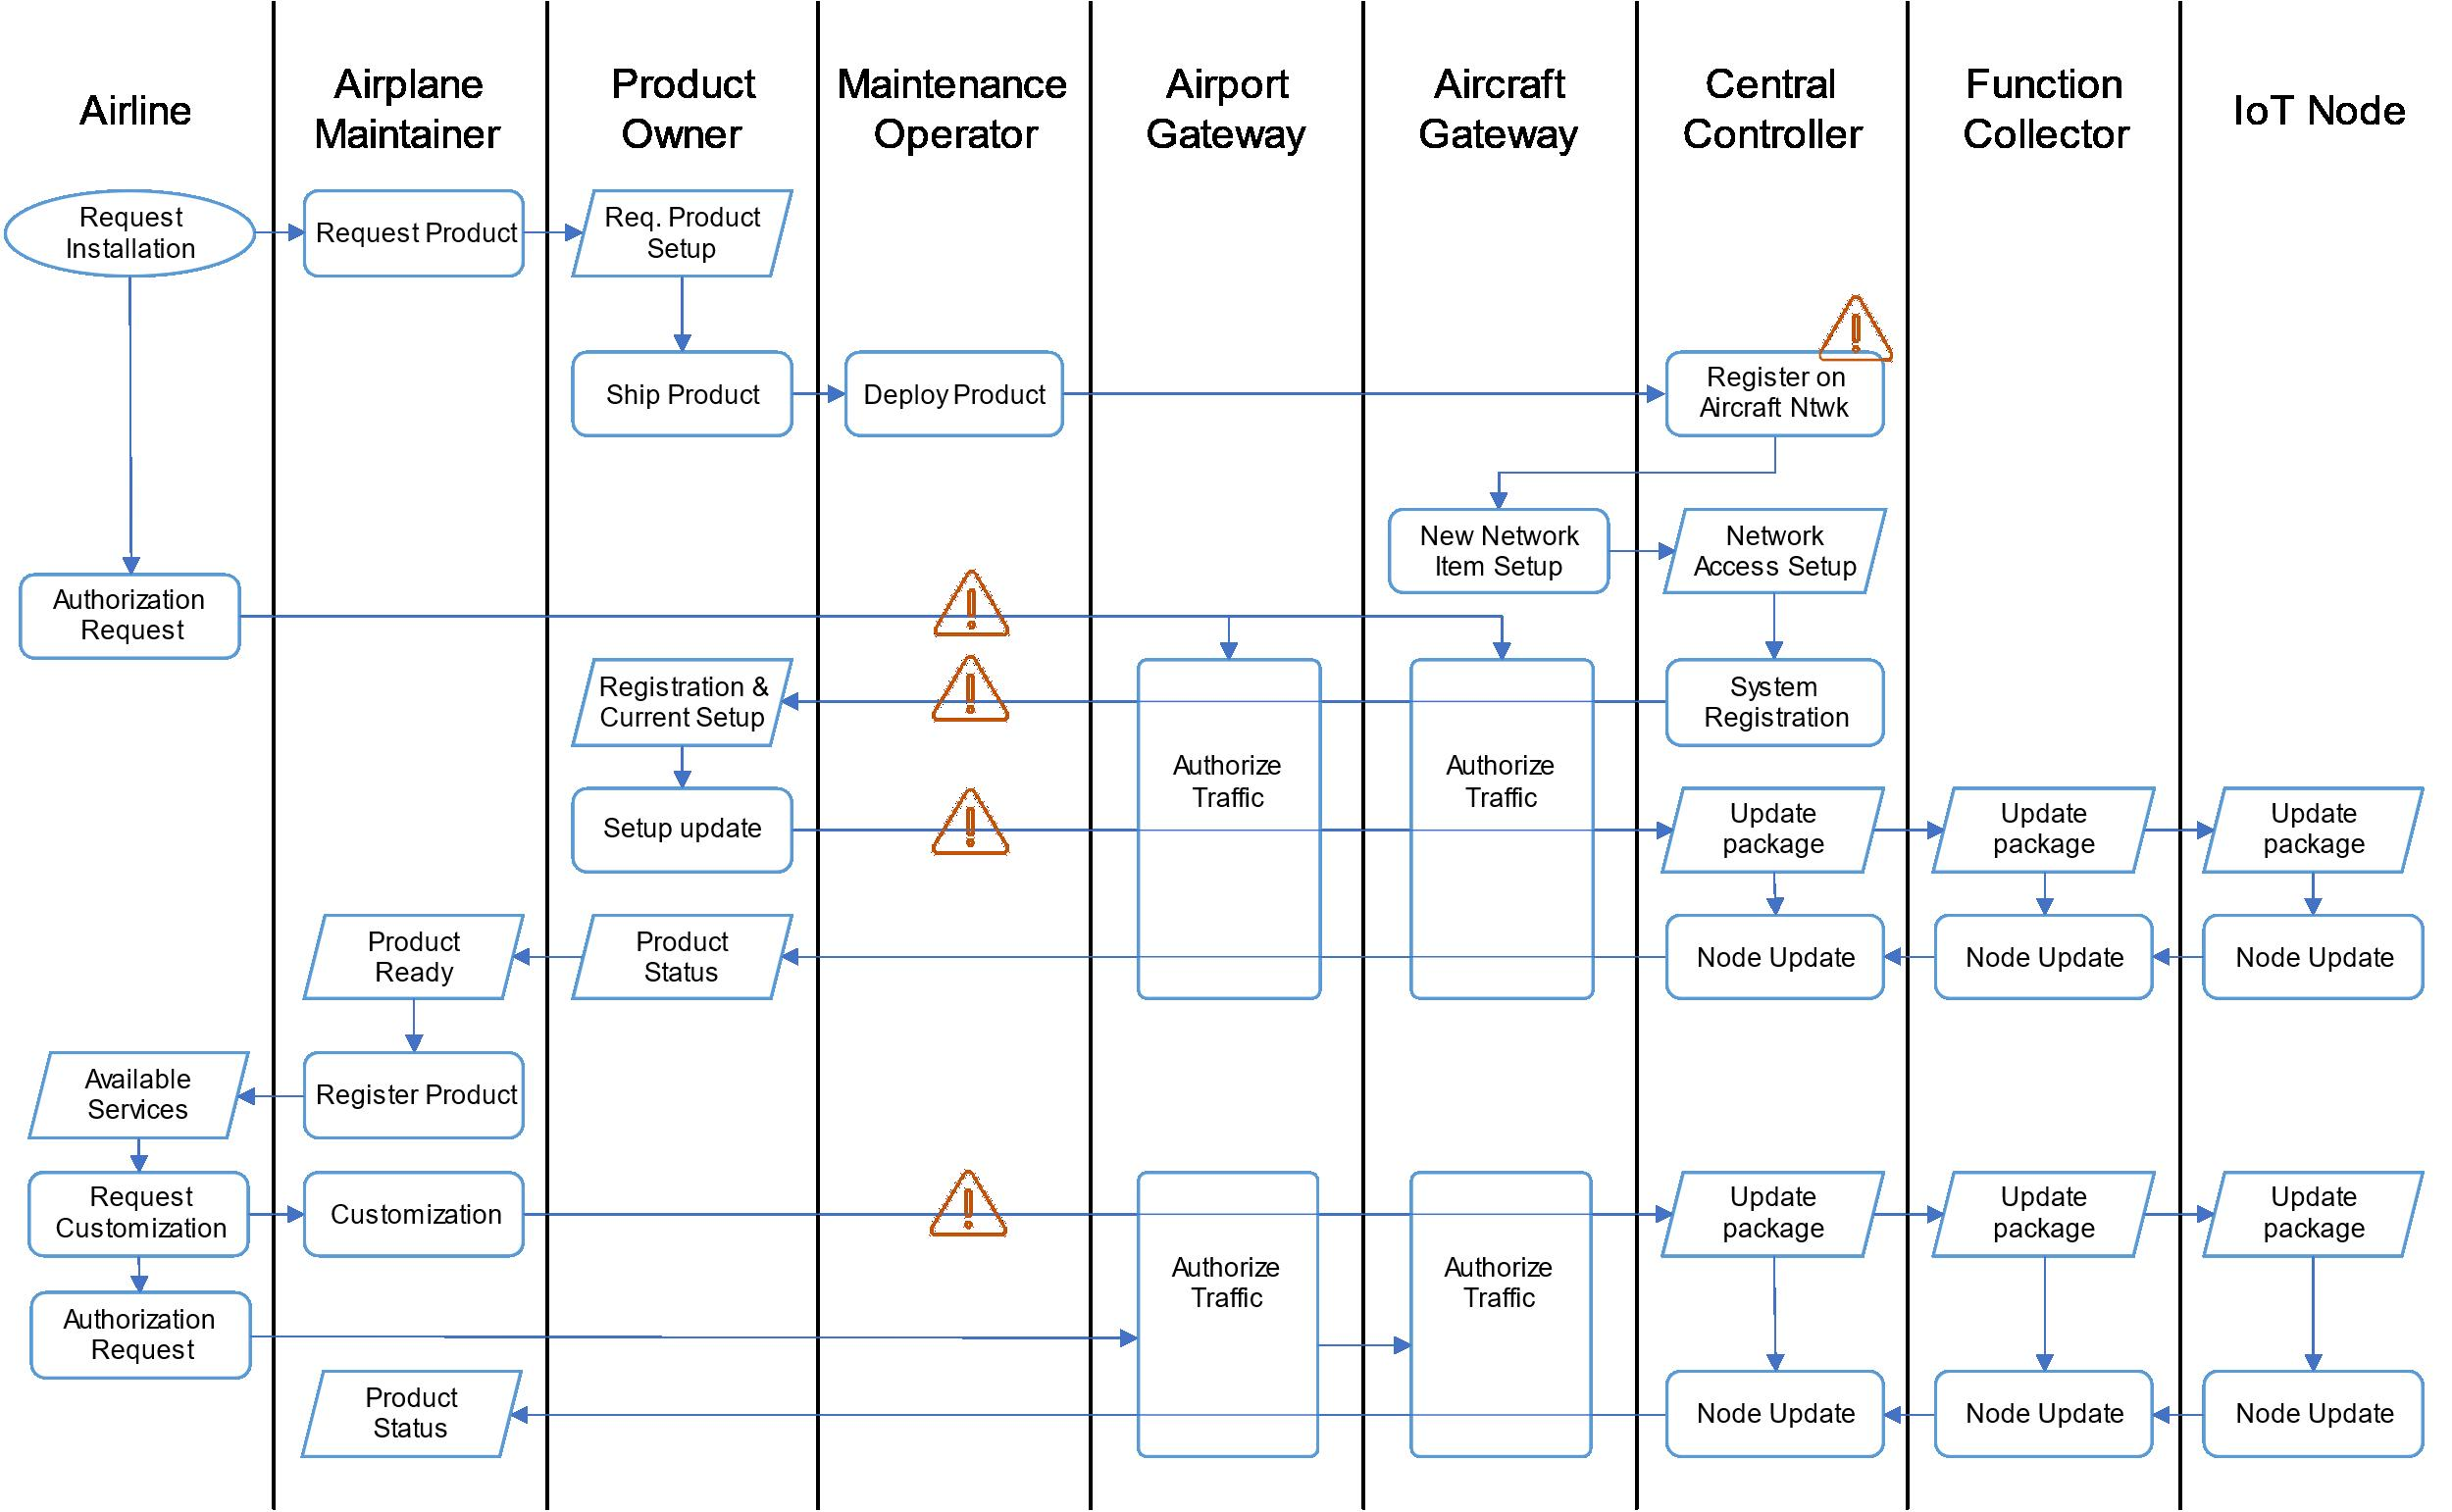
\includegraphics[width=0.95\textwidth]{figures/collins-s1-installation.jpg}
	\end{center}
	\caption{Collins Scenario 1: Device Installation}
	\label{fig:collins-s1-installation}
\end{figure}

\paragraph{Flow of Events}

The flow of events can be tracked in Figure~\ref{fig:collins-s1-installation} and is verbalized as follows:

\begin{itemize}
	\item Airline requests installation of new component to the Airplane Maintainer also issuing an authorization
	      request to Airport and Airplane gateways.
	\item The request is forwarded to the Product Owner and then to the Maintenance Operator, who oversees the
	      physical deployment of the product.
	\item Once connected, Central Controller registers on the Aircraft Network and receives required setup to
	      complete network access and system registration.
	\item Product Owner is now able to reach the CCS, push configuration and security updates to the Central
	      Controller, as well as the Function Collector and IoT nodes.
	\item After the update, the product is registered and the Airplane Maintainer can offer remote services to the
	      Airline.
	\item The Airline requests a customization of the CCS. It is performed by the Airplane Maintainer by pushing an
	      update package and/or modifying specific configurations as allowed by the Product Owner API for
	      Maintenance.
	\item The new product status is confirmed with a feedback message.
\end{itemize}

\subsubsection{Sub-Scenario 2: Component Replacement}

\begin{figure}
	\begin{center}
		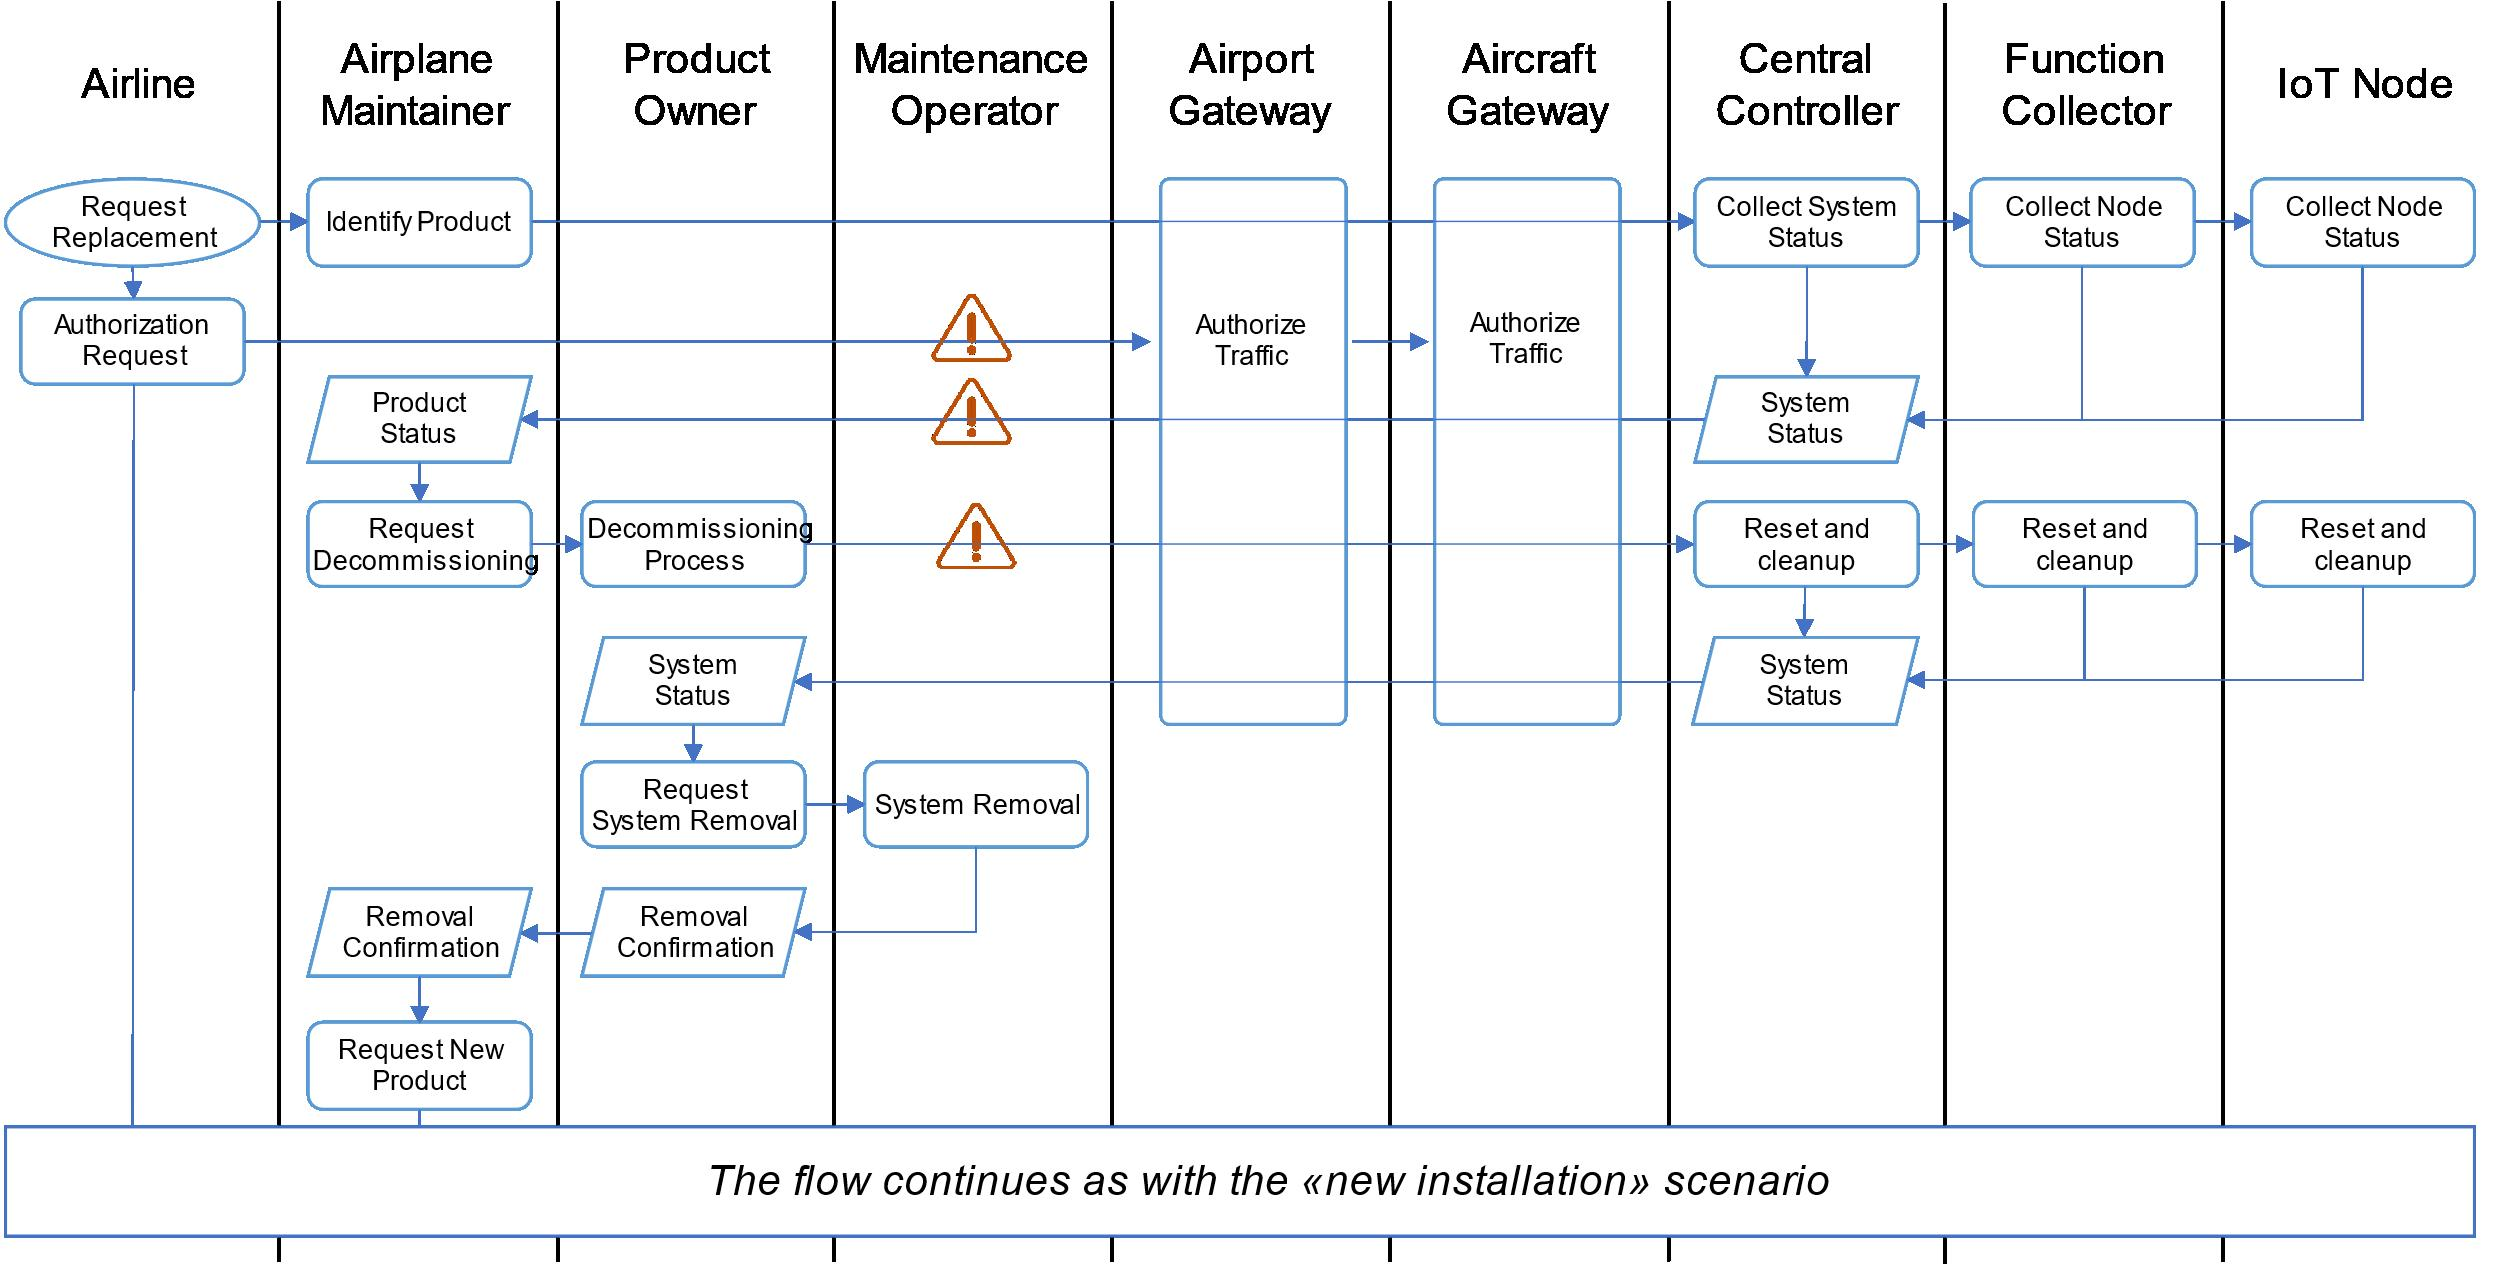
\includegraphics[width=0.95\textwidth]{figures/collins-s1-replacement.jpg}
	\end{center}
	\caption{Collins Scenario 1: Device Replacement}
	\label{fig:collins-s1-replacement}
\end{figure}

\paragraph{Flow of Events}

\begin{itemize}
	\item The Airline requests replacement of a component to the Airplane maintainer, also issuing an authorization
	      request to the Airport and Airplane Gateways.
	\item The Airplane Maintainer identifies the target product (location) and collects latest system status.
	\item The Airplane Maintainer issues a decommissioning request to the Product Owner and starts the
	      decommissioning process, which causes a reset and cleanup of all the nodes that will be replaced.
	\item After remote reset and clean-up, product owner requests the Maintenance Operator to physically remove the
	      system from the cabin.
	\item The product is then unregistered and can be dismissed.
	\item The remaining part continues with the 'New installation process flow'
\end{itemize}

\subsubsection{Post-Condition}

After completion of the Installation Scenario, following post-conditions need to be met:

\begin{itemize}
	\item New component is deployed in the CCS, integrated into the network, updated with latest security patches
	      and configured by the Airline for their specific needs.
	\item Component is securely onboarded in the CCS, unique identity and certificates are dispatched for
	      authentication.
	\item Regarding the configurations, their integrity is verified and confidentiality has been preserved.
\end{itemize}

\subsubsection{Attack Scenario}

As an alternative flow of events, i.e., in an attack scenario, highlighted by the yellow triangles in
Figure~\ref{fig:collins-s1-installation} and Figure~\ref{fig:collins-s1-replacement} following points were identified:

\begin{itemize}
	\item Attacker can inject malicious payloads in place of the intended one, (confidential) credentials provided
	      to the Central Controller for network access and authentication ca be stolen.
	\item IP sensitive data can be leaked by the Airplane Maintainer when retrieving the system status.
	\item The integrity of maintenance/reset/cleanup procedures can be compromised.
\end{itemize}

% subsection Installation of Connected Cabin Systems (end)

\subsection{System Operation and Monitoring} % (fold)
\label{sub:System Operation and Monitoring}

\begin{table}
	\caption{Actors involved operations}
	\label{tab:Actors involved}
	\begin{center}
		\begin{tabular}{ |p{2.5cm}|p{2.5cm}|p{2.5cm}|p{2.5cm}|p{2.5cm}| }
			\hline
			Airline & Airplane Maintainer & Product Owner & Maintenance Operator & Passenger, Attendant, Pilot \\
			\hline
			X       & X                   & X             & -                    & X                           \\
			\hline
		\end{tabular}
	\end{center}
\end{table}

\begin{table}
	\caption{Lifecycle stages involved}
	\label{tab:Lifecycle stages involved operations}
	\begin{center}
		\begin{tabular}{ |c|c|c|c|c| }
			\hline
			Bootstrapping & Operation & Update & Repurposing & Decommissioning \\
			\hline
			-             & X         & X      & -           & -               \\
			\hline
		\end{tabular}
	\end{center}
\end{table}

\subsubsection{Goals}

The goals of System Operations and Monitoring incorporate following points:

\begin{itemize}
	\item Periodic collection of data from airplane.
	\item Data offload/upload to ground stations for performance monitoring, optimization and PHM operations.
	\item Attendants interact with CCS through a HMI
	\item CCS Information is collected and stored in Gateway.
	\item A limited set of predefined reconfigurations may be performed on plane, when requested by Airline,
	      Maintainer or product owner.
\end{itemize}

\subsubsection{Pre-conditions}
\begin{itemize}
	\item Maintainers have established remote secure connection with the aircraft (wireless or wired) through the
	      airport infrastructure.
	\item Passengers/Attendants/Pilots can interact through HMI or are connected through other devices e.g., through
	      WiFi (possibly in the sense of bring you own device, BYOD).
	\item Device bootstrapping, enrollment, configuration, provisioning are completed for all devices, that are
	      (statically) part of the network.
	\item IoT devices are equipped with sensors to collect and store data that are then forwarded to their root
	      controller.
	\item Devices can securely store and transmit collected data.
\end{itemize}

\subsubsection{Flow of Events}

\ref{fig:collins-s2-data-collection-reconfig}
\ref{fig:collins-s2-data-unload-remote-analysis}
\ref{fig:collins-s2-data-load-remote-config}

\begin{itemize}
	\item IoT devices collect data during airplane operations, see Figure \ref{fig:collins-s2-data-collection-reconfig}
	\item Data is securely stored on-board, see Figure \ref{fig:collins-s2-data-collection-reconfig}
	\item Local computations over critical and non-critical data are executed in separate environments to reconfigure
	      the airplane/flight, see Figure \ref{fig:collins-s2-data-collection-reconfig}
	      \textbf{What is meant by this?}
	\item Remote entities are authenticated and a connection is established with the aircraft network through the
	      gateway, see Figure \ref{fig:collins-s2-data-load-remote-config}
	      \textbf{What Gateway? We are basically in flight so shouldn't we be disconnected? Otherwise this is
		      a scenario for Roaming}
	\item Data is downloaded from plane to ground
	\item In case of an Airplane fleet, Collective Analysis is performed, see Figure
	      \ref{fig:collins-s2-data-unload-remote-analysis}
	\item Upload new data and configurations, from ground to plane
	\item Data authenticity and integrity are verified before updating the configurations on the plane.
\end{itemize}

% \subsubsection{Sub-Scenario 1: Data Collection and Local Reconfiguration}
\begin{figure}
	\begin{center}
		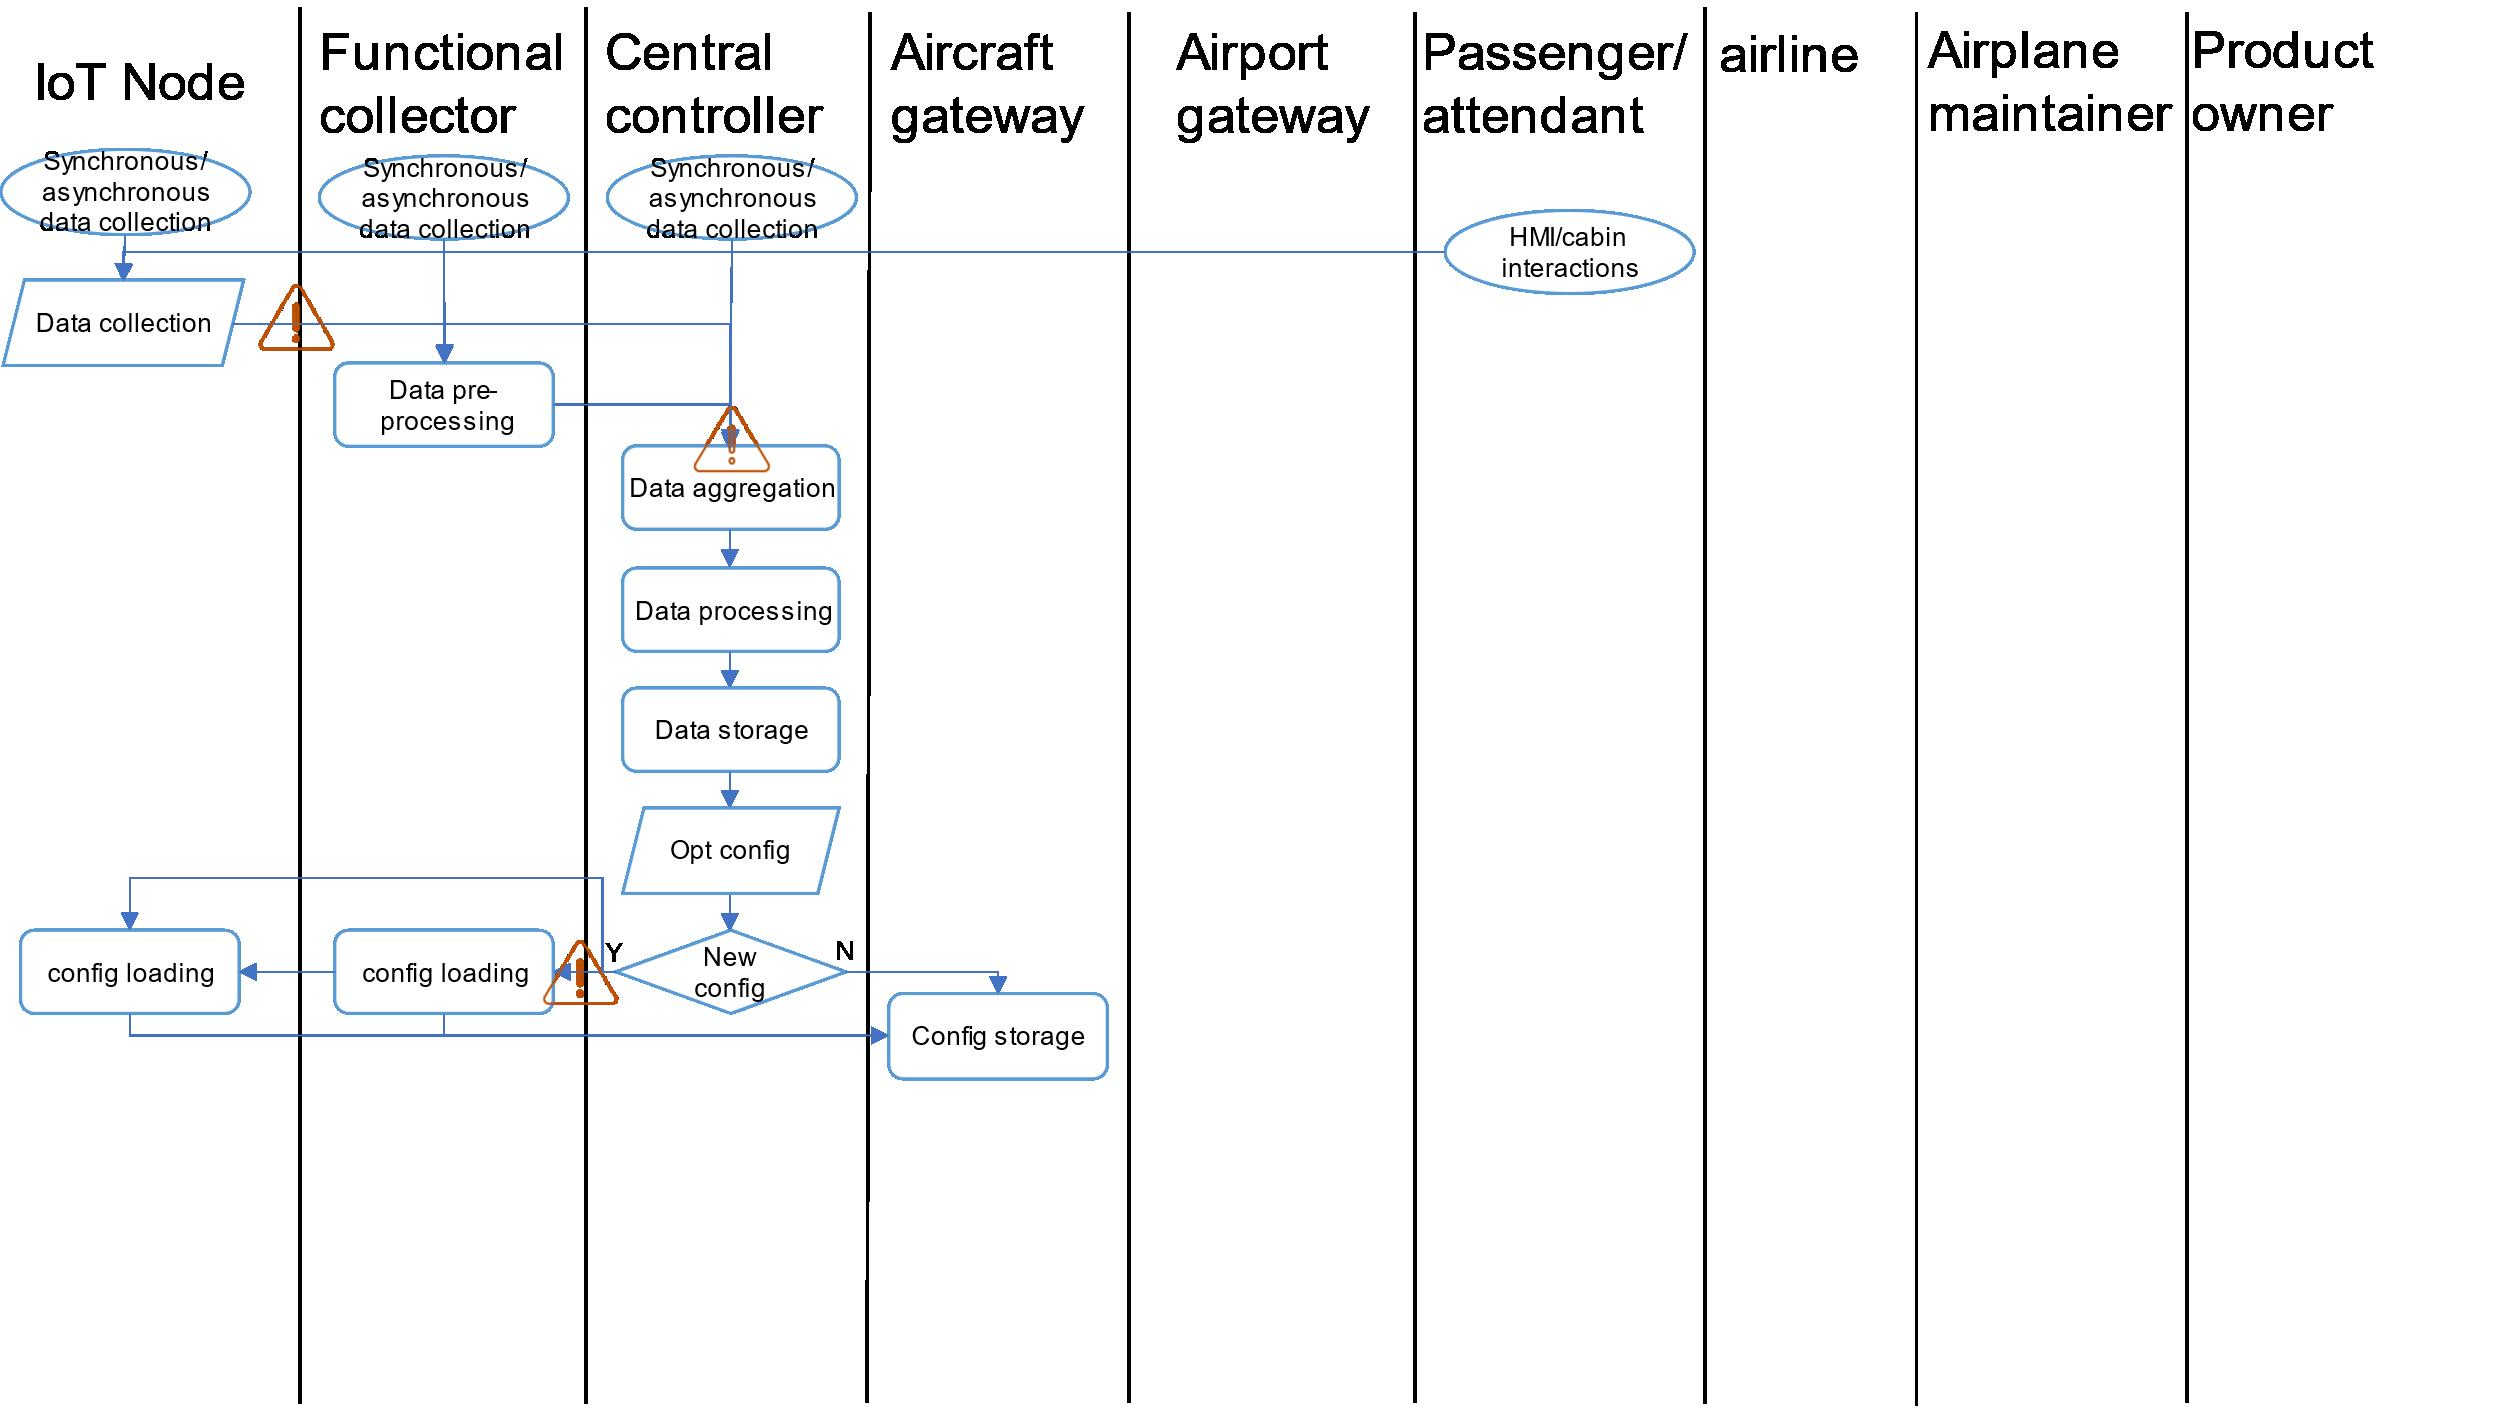
\includegraphics[width=0.95\textwidth]{figures/collins-s2-data-collection-reconfig.jpg}
	\end{center}
	\caption{Collins Scenario 2.1: Data Collection and Local Reconfiguration}
	\label{fig:collins-s2-data-collection-reconfig}
\end{figure}

% \subsubsection{Sub-Scenario 2: Data Unload and Remote Analysis}
\begin{figure}
	\begin{center}
		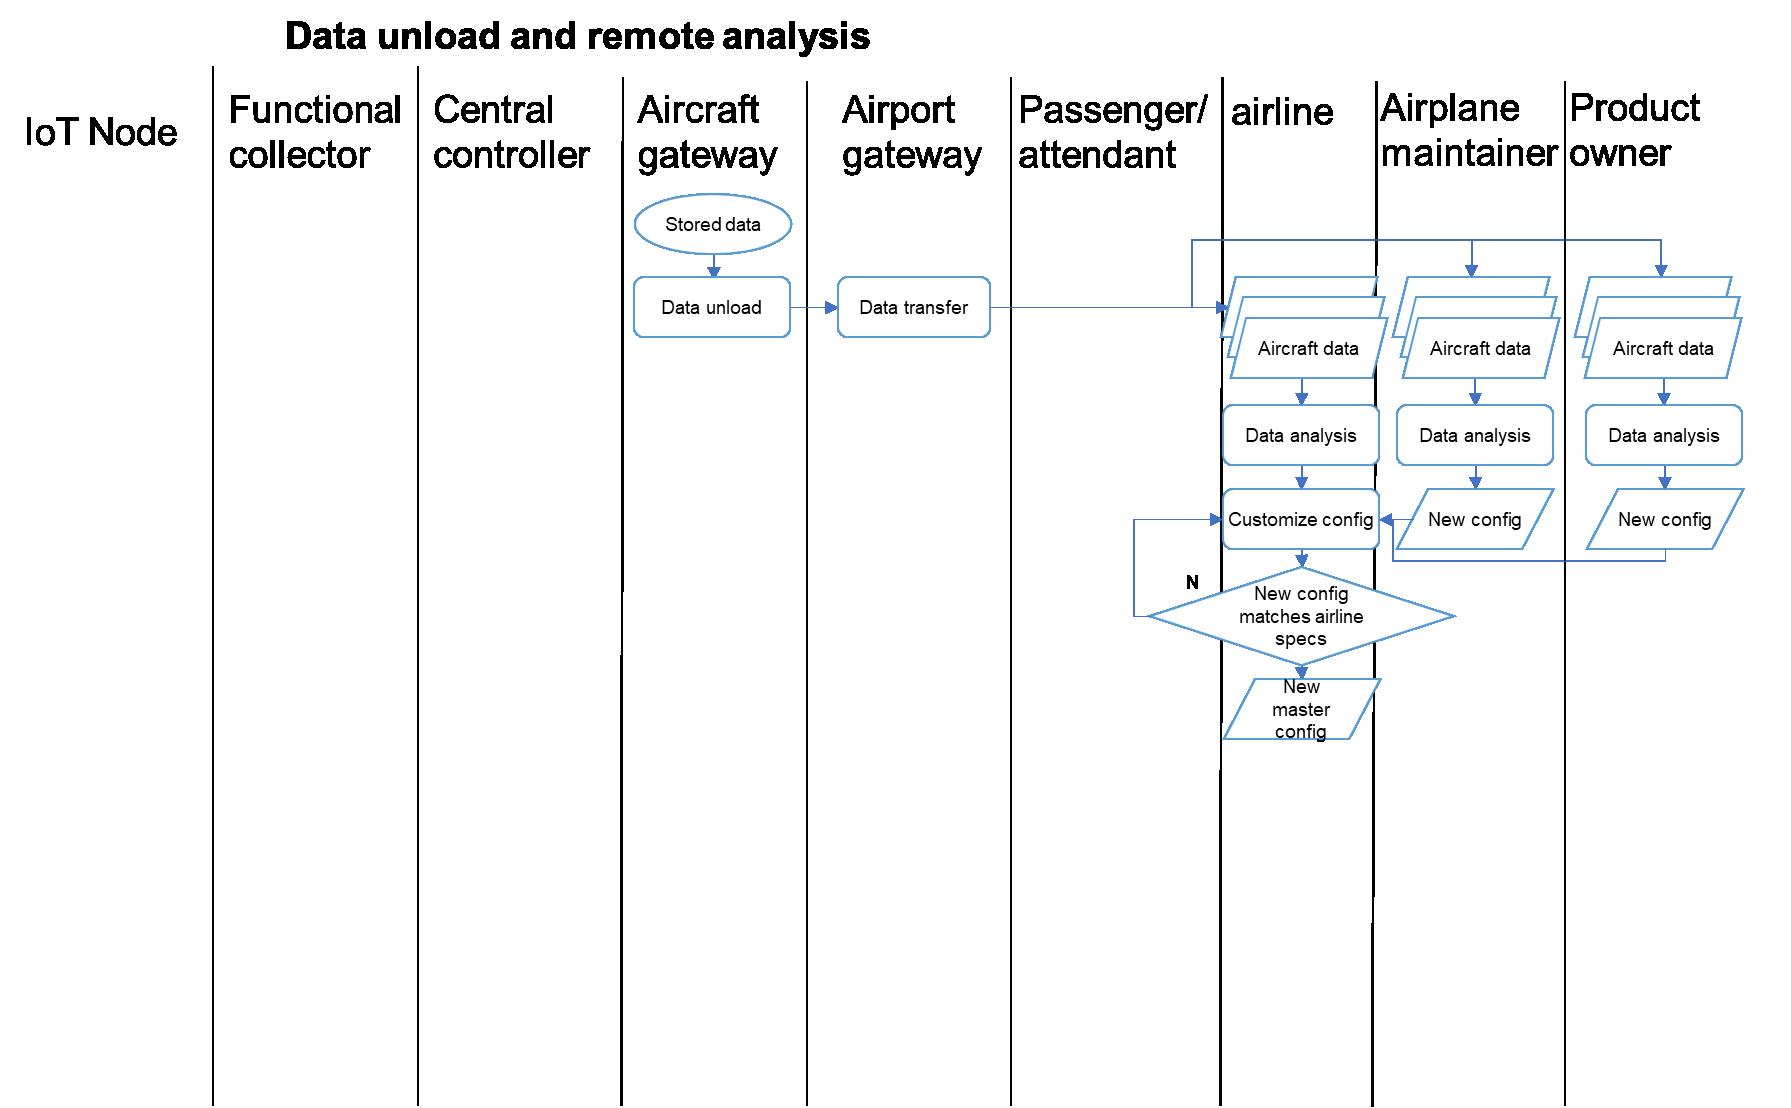
\includegraphics[width=0.95\textwidth]{figures/collins-s2-data-unload-remote-analysis.jpg}
	\end{center}
	\caption{Collins Scenario 2.2: Data Unload and Remote Analysis}
	\label{fig:collins-s2-data-unload-remote-analysis}
\end{figure}

% \subsubsection{Sub-Scenario 3: Data Load from Remote Config}
\begin{figure}
	\begin{center}
		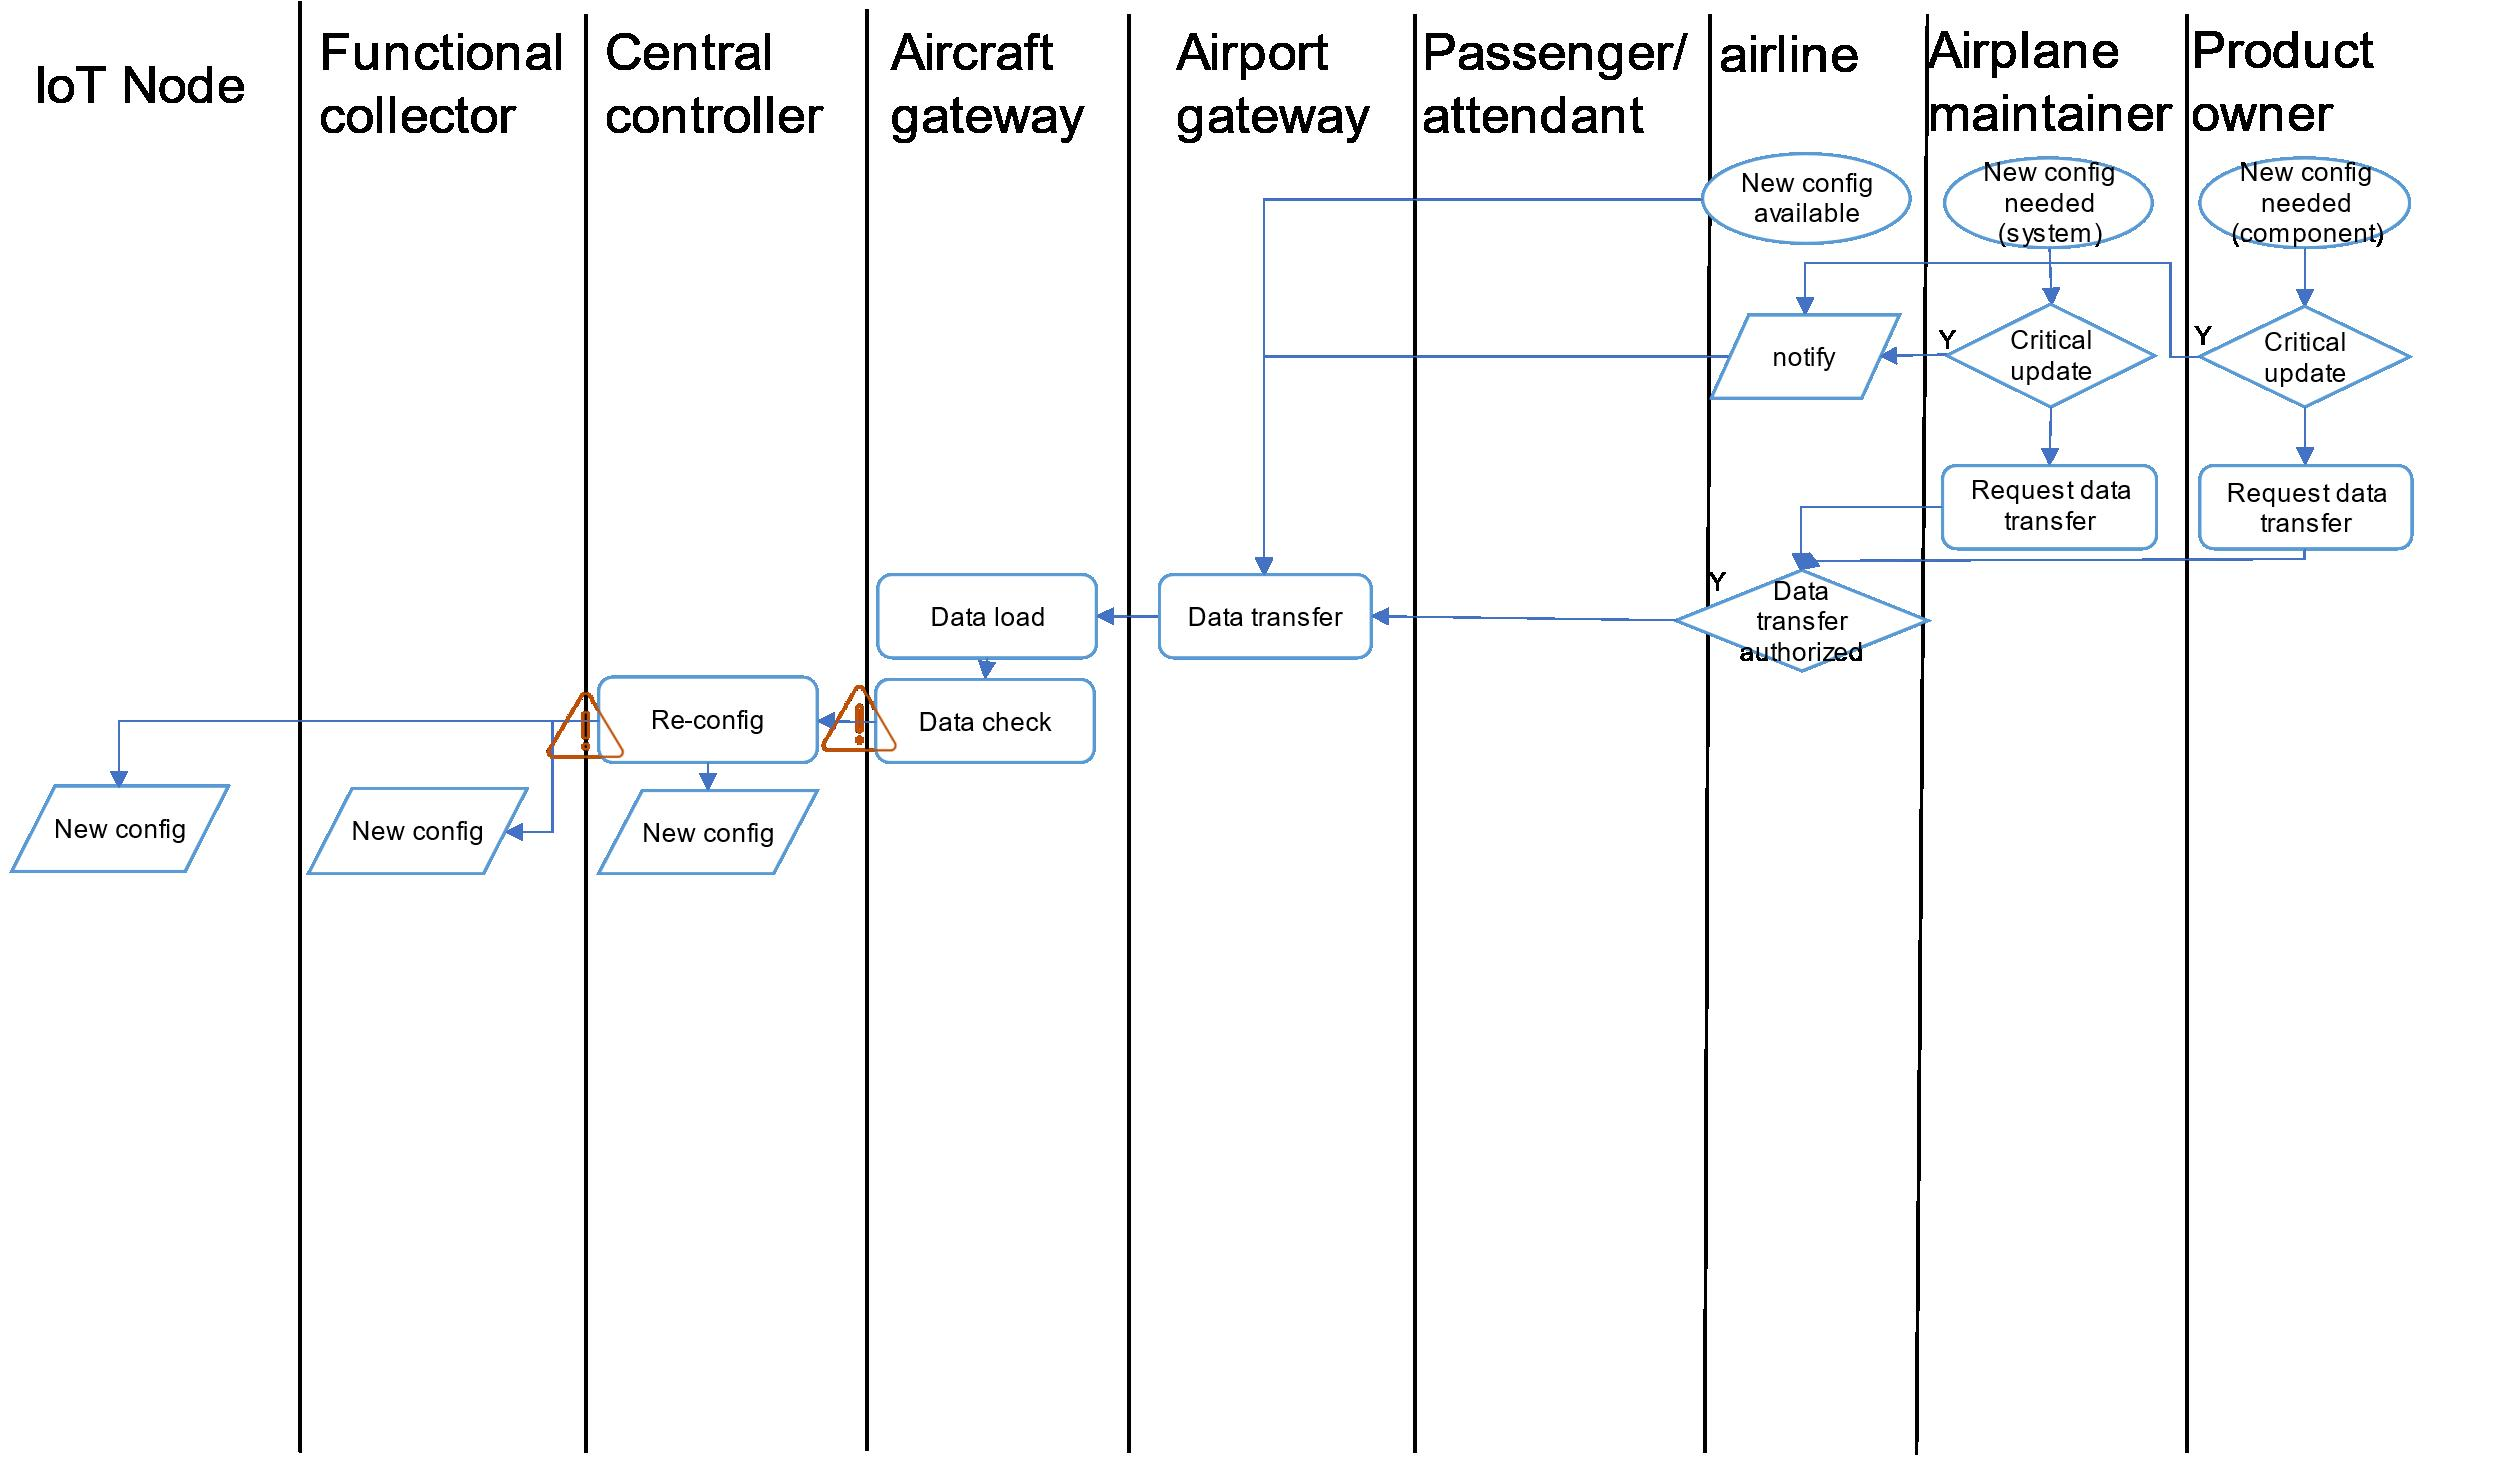
\includegraphics[width=0.95\textwidth]{figures/collins-s2-data-load-remote-config.jpg}
	\end{center}
	\caption{Collins Scenario 2.3: Data Load and Remote Reconfiguration}
	\label{fig:collins-s2-data-load-remote-config}
\end{figure}

\subsubsection{Post-Conditions}

After any of the sub-scenarios from Figures \ref{fig:collins-s2-data-collection-reconfig},
\ref{fig:collins-s2-data-unload-remote-analysis}, \ref{fig:collins-s2-data-load-remote-config}, the following
post-conditioned need to be met:

\begin{itemize}
	\item A new configuration, computed either locally or through the remote connection with the operations center
	      is available.
	\item Data from the aircraft are available for further analysis of Airline, Maintainer or Product Owner.
	\item For the configurations, integrity is verified, and confidentiality has been preserved (as it could
	      involve IP issues) in the process.
	\item For the data, in addition to integrity and confidentiality, it is important to also ensure availability
	      (to detect early sings of potential problems).

\end{itemize}

\subsubsection{Attack Scenario}

As an alternative flow of events, where an attack might happen, the main entry point is through the WiFi access point.
A rogue device could inject false data, configurations or software to facilitate subsequent attacks or even cause system
unavailability or device malfunctioning.
Alternatively in stealth mode, sensitive information could be captures and could be used to perpetrate other attacks.

% subsection System Operation and Monitoring (end

\subsection{LRU Replacement and Repurposing} % (fold)
\label{sub:LRU Replacement and Repurposing}

Akin to Scenario 1 in Subsection \ref{sub:Installation of Connected Cabin Systems} in this Scenario we also consider
similar steps to replace existing devices, with the difference, that the devices that replace the broken devices were
not exactly meant for this situation.

\begin{table}
	\caption{Actors involved}
	\label{tab:Actors involved lru}
	\begin{center}
		\begin{tabular}{ |p{2.5cm}|p{2.5cm}|p{2.5cm}|p{2.5cm}|p{2.5cm}| }
			\hline
			Airline & Airplane Maintainer & Product Owner & Maintenance Operator & Passenger, Attendant, Pilot \\
			\hline
			X       & X                   & X             & X                    & -                           \\
			\hline
		\end{tabular}
	\end{center}
\end{table}

\begin{table}
	\caption{Lifecycle stages involved}
	\label{tab:Lifecycle stages involved lru}
	\begin{center}
		\begin{tabular}{ |c|c|c|c|c| }
			\hline
			Bootstrapping & Operation & Update & Repurposing & Decommissioning \\
			\hline
			-             & -         & X      & X           & X               \\
			\hline
		\end{tabular}
	\end{center}
\end{table}

\subsubsection{Goals}

The goal of this scenario is to quickly replace a malfunctioning Central or Functional Controller, but a LRU is not
directly available. To minimize downtime, a spare LRU is retrieved from the same manufacturer and repurposed to the
specific target system. Airline, Airplane Maintainer, Product Owner, and Maintenance Operator are all involved to take
care of different steps in the process.

\subsubsection{Pre-Conditions}

Following pre-conditions must be met:

\begin{itemize}
	\item Actors involved can establish remote secure connection with aircraft.
	\item Airport has a spare LRU, that is compatible with CCS.
	\item The Maintenance Operator is provided access to the airplane and to the maintenance ports.
\end{itemize}

\subsubsection{Flow of Events}
\begin{figure}
	\begin{center}
		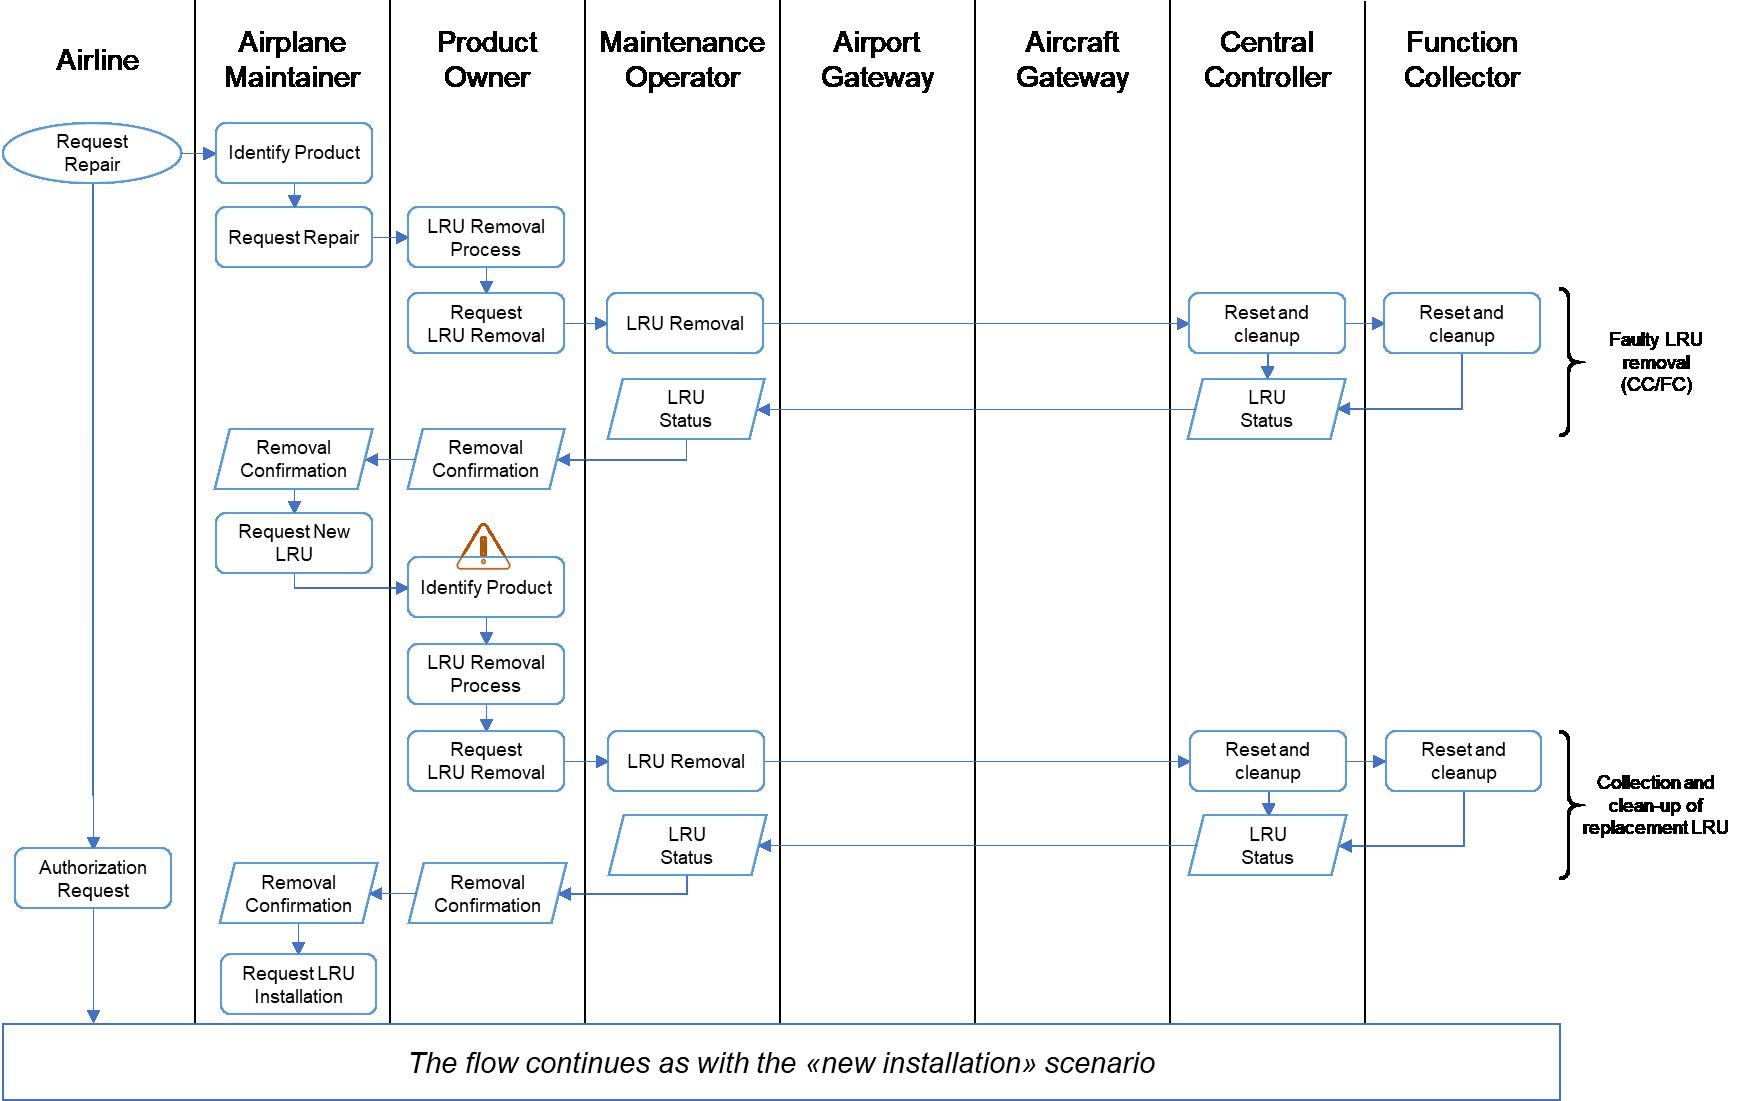
\includegraphics[width=0.95\textwidth]{figures/collins-s3-lru.jpg}
	\end{center}
	\caption{Collins Scenario 3: LRU Replacement}
	\label{fig:collins-s3-lru}
\end{figure}

\begin{itemize}
	\item The Airline requests to the Airplane Maintainer the repair of a cabin system, issuing and authorization
	      request to the Airport/Airplane gateways for following remote software update operations.
	\item The Airplane Maintainer identifies the target product, including its location, and the failure condition
	      then requests repair to Product Owner.
	\item The Product Owner starts the removal process of the LRU, including reset and cleanup
	\item Failed LRU removal executed locally by Maintenance Operator (also in charge of reset and cleanup)
	\item Product owner informs Airplane Maintainer of the removal and receives information of available replacement
	      LRUs.
	\item The replacement LRU shall be available from a remote location.
	\item The remaining flow proceeds as in Scenario 1 in Subsection \ref{sub:Installation of Connected Cabin Systems}

\end{itemize}

\subsubsection{Post-Conditions}
\begin{itemize}
	\item A new LRU  is deployed, integrated into network, updated with latest security patches and configured by
	      the Airline for specific needs
	\item CCS is registered with unique identifier and certificates are dispatched for authentication.
	\item For the configuration, integrity is verified and confidentiality has been preserved (for IP protection)
	      in the process
\end{itemize}

\subsubsection{Attack Scenario}

Attacks follow same pattern as in Subsection \ref{sub:Installation of Connected Cabin Systems} from Scenario 1.
An attacker can inject malicious software or a counterfeit LRU through the supply chain.
% subsection LRU Replacement and Repurposing (end)

\begin{figure}
	\begin{center}
		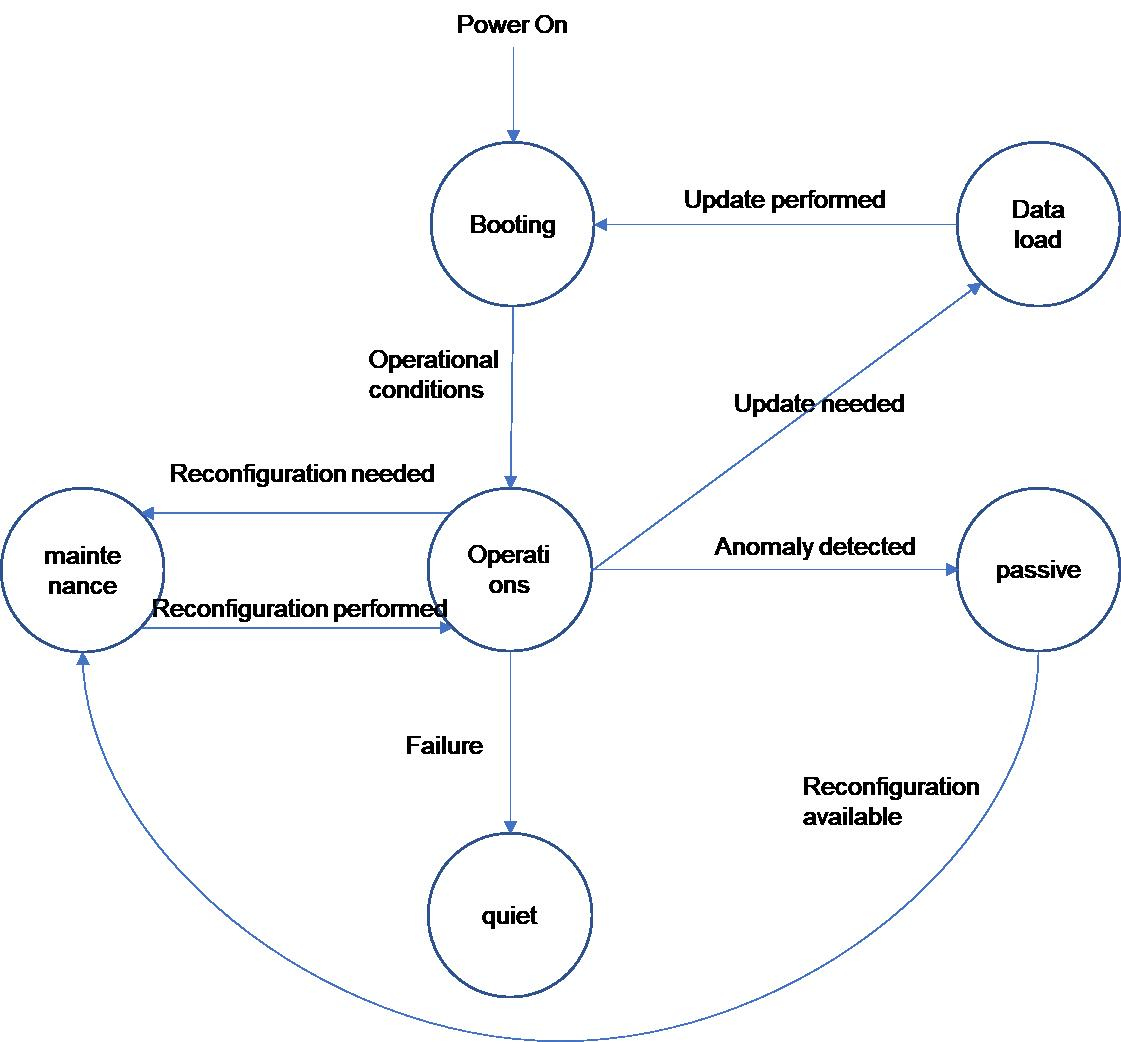
\includegraphics[width=0.95\textwidth]{figures/collins-opmodes.jpg}
	\end{center}
	\caption{Collins Operation Modes for an On-Board Device}
	\label{fig:collins-opmodes}
\end{figure}

% section Scenarios (end)

\section{Cybersecurity Assessment} % (fold)
\label{sec:Cybersecurity Assessment}

\begin{figure}
	\begin{center}
		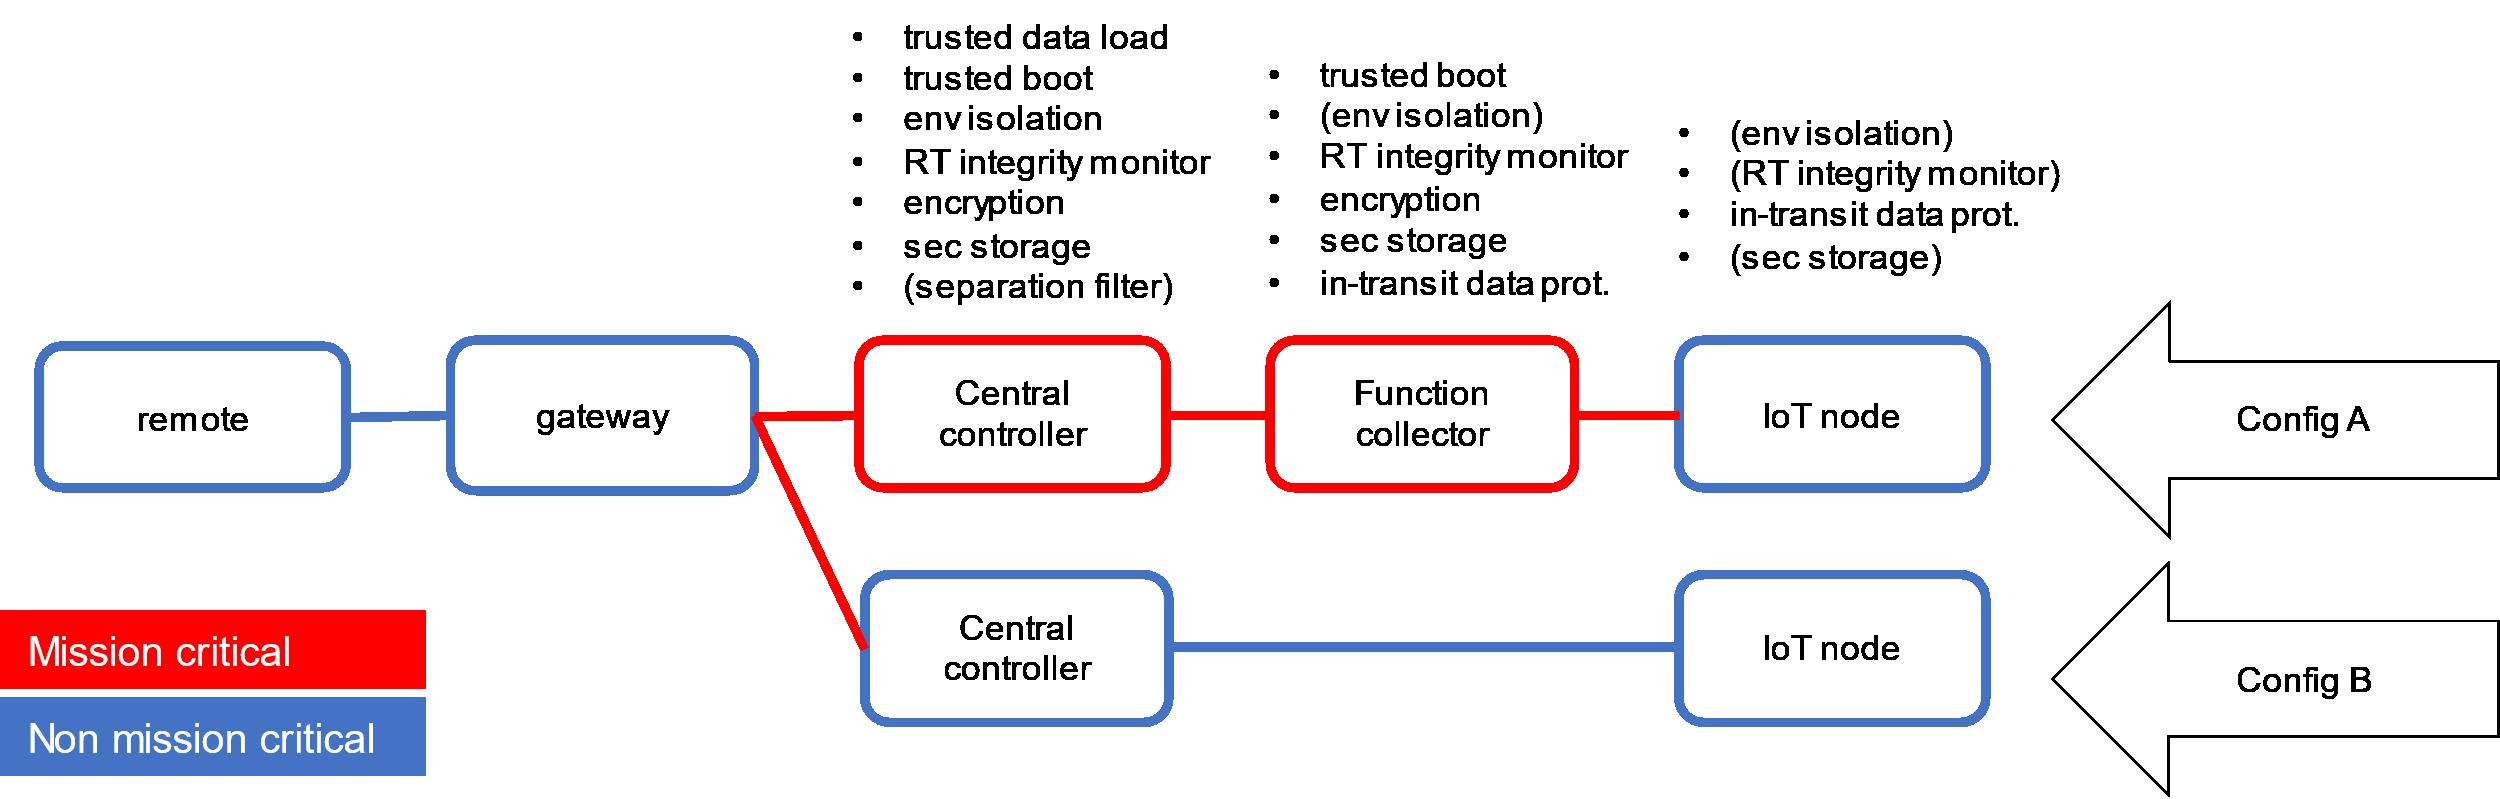
\includegraphics[width=0.95\textwidth]{figures/collins-sec-feat.jpg}
	\end{center}
	\caption{Collins Desired Security Features for the Different CCS Components}
	\label{fig:collins-sec-feat}
\end{figure}

The CERTIFY \cite{certifyproject2023} project describes following security levels:

\begin{itemize}
	\item Basic: Focus on common and simple cyber threats. User authentication, access controls and basic security
	      configuration.
	\item Substantial: More robust security measures including intrusion detection systems, IDS, incident response
	      plans and periodic security assessment.
	\item High: Requires organizations to establish comprehensive and proactive cybersecurity programs. Further
	      advanced security measures, network segmentation, encryption, continuous monitoring and regular
	      vulnerability assessments are needed. Threat intelligence sharing and regular security audits are also in
	      order.
\end{itemize}

Our use case, CCS, falls into the category of level \textit{HIGH}, as from a cybersecurity viewpoint the aircraft cabin
is considered a highly volatile and highly targeted environment.

% section Cybersecurity Assessment (end)
